\documentclass[pdftex,12pt,a4paper]{article}

\usepackage[T1]{fontenc}
\usepackage[utf8]{inputenc}
\usepackage[lined,boxed,linesnumbered,commentsnumbered]{algorithm2e}
\usepackage{amsmath}
\usepackage{hyperref}
\usepackage{graphicx}


\begin{document}

\title{
	\Large \textbf{Algorithms for social networks} \\
	\textsf{Report of the project \emph{PageRank}}
}
\author{Andreea Beica \and Baptiste Lefebvre}
\date{21 january 2014}

\maketitle


\section{Presentation}

The PageRank algorithm, alongside a family of Google related technologies, represent a unique approach to the task of information handling and data retrieval, their scope and possible applications extending far beyond the search box of Google.com.

More specifically, PageRank is a method of assessing the importance of a web page based upon its relationship with to other pages. As presented in the Abstract of the original patent, it is :

\vspace{10pt}

\begin{centering}
\textbf{"A method [that] assigns importance ranks to nodes in a linked database, such as any database of documents containing citations, the world wide web or any other hypermedia database."}
\end{centering}
\vspace{10pt}

What makes PageRank's importance extend beyond the scope of a simple search engine, is that when applied to all of the web pages within the Google index and after analysing the output, it constitutes an accurate of user behavior probability, as well as offering a completely objective measure measure of a web page's importance, all of which is computed mathematically and without human interference. 

In the words of its authors:

\vspace{10pt}

\begin{centering}
\textbf{"PageRank can be thought of as a model of user behavior. We assume there is a \emph{random surfer} who is given a web page at random and keeps clicking on links, never hitting \emph{back} but eventually gets bored and starts on another random page. The probability that the random surfer visits a page is its PageRank."}
\end{centering}
\vspace{10pt}

When compared to already existing text-based search engines, which relied primarily on information contained within given page (such as titles with a high keyword density, search terms placed near the top of the document, or having the highest density of the search term) to determine its relevance to a search query - and so which could be easily manipulated and ultimately unreliable, the PageRank approach aimed to provide a vast improvement in the quality and accuracy of document retrieved by a search engine in response to a search  phrase query. This goal would be accomplished by:

\begin{itemize}
\item objectively evaluating the importance of web pages and assigning corresponding ranks
\item using the rank information of said web pages to help determine relevance and placement withing a Search Engine Result Page
\end{itemize}

The formal description of the PageRank formaula is as follows (as described by its authors):

\vspace{10pt}


\textbf{"We assume page A has pages T1...Tn which point to it (i.e., are citations).
The parameter d is a damping factor which can be set between 0 and 1. We
usually set d to 0.85.
Also C(A) is defined as the number of links going out of page A. The
PageRank of a page A is given as follows:}

\vspace{10pt}

\begin{centering}
\textbf{PR(A) = (1-d) + d (PR(T1)/C(T1) + ... + PR(Tn)/C(Tn))}
\end{centering}
\vspace{10pt}

\textbf{Note that the PageRanks form a probability distribution over web pages, so the sum of all web pages' PageRanks will be one."}

\vspace{10pt}

We break down the formula of PR(A), for clarification purposes:

\begin{itemize}
\item \textbf{PR(Ti)} = the PageRank of $i^{th}$ page pointing to page A
\item \textbf{PR(Ti)/C(Ti)} = any linking web page divides the weight of its vote evenly amongst all of the votes that it gives
\item \textbf{d} = every vote is added together to determine the PageRank value of page A; however, in order to prevent a \emph{combined strength} effect from over inflating PR(A), the final value is multiplied by a \emph{damping factor}, of usually .85
\item \textbf{(1-d)} = this ensures that the sum of all web pages' PageRank will be 1, by adding the amount lost by the damping factor back in ; thus, every web page will have at least that minimal value
\end{itemize}

The purpose of this project is to implement different versions of the PageRank and test it on a set of Wikipedia set of downloaded pages.


\section{Project architecture}

In order to apply the PageRank formula to the task of word-based web search, we had to simulate crawling and indexing the Web. 

Crawling the web proved to be a difficult task (see Section 5), so we resumed to downloading static HTML dumps of all pages of Wikipedia for a certain language (e.g., Table 1 contains results for the Wikipedia entries of \emph{rumantsch}, a romance language dialect spoken in Switzerland, for which the number of articles was reasonable enough to ensure the memory would be sufficient when running the algorithms - around 6000 articles) and resume to crawling and indexing these pages.
\vspace{10pt}

The architecture and algorithms used for indexing were inspired by the ones presented in \cite{1}:

\begin{itemize}
\item \textbf{Parsing}: in our file system, which contains the web pages, we parse each page, in order to construct the two structures indispensable to computing the PageRank: the \emph{inverted index} and the \emph{pointsTo} table - a table containing all the hyperlinks between pages (the PageRank formula is based on this graph-like vision of the web pages, in which a hyperlink from page A to page B is viewed as a "vote of trust" of sorts for page B)
\item \textbf{The inverted index}: used for quick lookup when one makes a query, our inverted index retains, for every word, a list of documents in which it appears, each entry in the list containing different informations like the docID, the number of occurences of the word,whether it appears in the document's title or not (see Figure 1).

\end{itemize}

\begin{figure}[h]
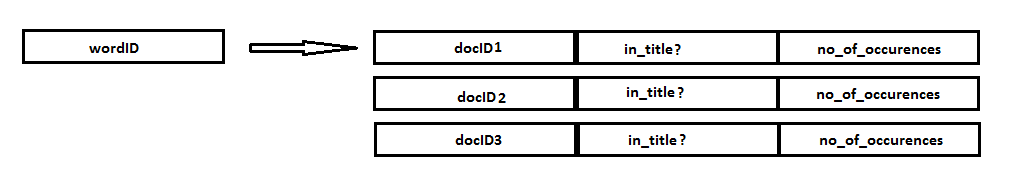
\includegraphics[width=0.8\textwidth]{index.png}
\caption{Inverted index}
\end{figure}

At the end of the parsing phase, we create both the graph of hyperlinks which will be used as input for the PageRank formula, as well as the inverted index, which is used in the case of a query.

\subsection{The IR score}

The IR (integrated reasoning) score is determined by the emphasis and weighted position of the specific terms used in a document, then used to compute the \emph{actual relevance} of each page in order to provide pages that are relevant to the terms of a specific search. This \emph{'actual relevance'} is computed by multiplying the IR score of each page to its PageRank value, to give a divisive value for how important each page is (we use multiplication because using addition would result in pages that are unrelated to the search terms ending up with a higher ranking in the search results returned from the query).

For now, the IR score we compute is a straightforward (and maybe simplistic) formula: if the search word appears in a document's title, its IR score is 2$*$n, else its IR score is simply n, where n denotes the number of occurences of the search word in the document.

\subsection{Searching}

For simplicity purposes, we limited our search (for the time being, at least), to \emph{single word queries}. The sketch of the algorithm in the case of a single word query (and assuming the PageRanks are computed for every page) is as follows:
\begin{enumerate}
\item  Look up the query word in the inverted index and retrieve the corresponding document list
\item Based on the information contained in the inverted index, compute the IR score for each document 
\item For each document, combine its IR score and its PageRank in order to give the document a final rank
\item Sort documents and return first \emph{k} 
\end{enumerate}





\section{Algorithms}

Three methods have been selected to implement the PageRank algorithm:
\begin{itemize}
\item iterative method
\item algebraic method
\item power method
\end{itemize}
This section details each of this method. They are all three based on the same input, a set $P = p_1, p_2, ..., p_n$ of HTML pages, with some hyperlinks between pages (i.e. $p_i \rightarrow p_j$), which defines a webgraph $G = \left(V, E\right)$ such that:
$$V = \{i \in N / p_i \in P\}$$
and:
$$E = \{\left(i, j\right) \in V \times V / p_i \rightarrow p_j\}$$
To make notations convenient, the following concepts are useful:
\begin{itemize}
\item $M\left(v\right)$ denotes the set of vertices that link to $v$ in $G$
\item $L\left(b\right)$ denotes the number of outbound edges for node $v$ in $G$
\item $A$ denotes the adjacency matrix of $G$ (i.e. $A_G\left[i\right]\left[j\right] \in \{0, 1\}$ and $A_G\left[i\right]\left[j\right] = 1 \Leftrightarrow \left(i, j\right) \in E$)
\end{itemize}

To calculate PageRank one must consider the following an essential equation:
$$ PageRank \left( i \right) = \frac{1 - d}{n} + d \sum\limits_{j \in M \left( i \right)} \frac{PageRank \left( j \right)}{L \left( j \right)}$$
where $d$ is the damping factor such that $d \in \left[ 0;1 \right] $. The first method iterates naively this equation on all the pages, many times, until convergence (note that convergence is not assume). With a little bit of linear algebra, one could find the equation verified by the PageRank vector. Essentially the problem of its calculation reduces to inverting a matrix and leads to the second method. Eventually with more advance linear algebra, \emph{Perron-Frobenius theorem}, one could find a more efficient algorithm with stands as the third method.

\subsection{Iterative method}
\IncMargin{1em}
\begin{algorithm}[H]
\SetKwInOut{Input}{Input}
\SetKwInOut{Output}{Output}
\BlankLine
\Indm
\Input{A webgraph $G$ with $n$ nodes}
\Output{An array $pr$ of size $n$}
\Indp
\BlankLine
\emph{// Initialization}\;
\For{$i \leftarrow 1$ \KwTo $n$}{
$pr'\left[i\right]\leftarrow\infty$\;
$pr\left[i\right]\leftarrow\frac{1}{n}$\;
}
\emph{// Iterations}\;
\While{$|pr-pr'|\geq\epsilon$}{
$pr' \leftarrow pr$\;
\For{$i \leftarrow 1$ \KwTo $n$}{
$pr\left[i\right]\leftarrow\frac{1-d}{N}+d\sum_{j\in M\left(i\right)}\frac{pr'[j]}{L\left(j\right)}$\;
}
}
\emph{// Renormalization}\;
$pr\leftarrow\frac{pr}{|pr|}$\;
\BlankLine
\caption{Iterative methods}\label{algo_iterative_method}
\end{algorithm}
\DecMargin{1em}

\subsection{Algebraic method}

\IncMargin{1em}
\begin{algorithm}[H]
\SetKwInOut{Input}{Input}
\SetKwInOut{Output}{Output}
\BlankLine
\Indm
\Input{A adjacency matrix $A$ of a webgraph $G$ with $n$ nodes}
\Output{An array $pr$ of size $n$}
\Indp
\BlankLine
\emph{// Initialisation}\;
\For{$j \leftarrow 1$ \KwTo $n$}{
\If{$L\left(j\right) \neq 0$}{
\For{$i \leftarrow 1$ \KwTo $n$}{
$A\left[i\right]\left[j\right]\leftarrow \frac{A\left[i\right]\left[j\right]}{L\left(j\right)}$
}
}
}
\emph{Computation}\;
$pr\leftarrow \left(dA-I\right)^{-1}\frac{1-d}{n}O$
\BlankLine
\caption{Algebraic method}\label{algebraic_method}
\end{algorithm}
\DecMargin{1em}

Additional notations have been used to describe the algebraic method, for a given integer $n$:
\begin{itemize}
\item $I$ denotes the identity matrix of size $n$
\item $O$ denotes the column vector of length $n$ containing only ones
\end{itemize}


\subsection{Power method}
\IncMargin{1em}
\begin{algorithm}[H]
\SetKwData{Left}{left}\SetKwData{This}{this}\SetKwData{Up}{up}
\SetKwFunction{Union}{Union}\SetKwFunction{FindCompress}{FindCompress}
\SetKwInOut{Input}{Input}\SetKwInOut{Output}{Output}
\BlankLine
\Indm
\Input{A webgraph $G$ with $n$ nodes}
\Output{An array $pr$ of size $n$}
\Indp
\BlankLine
\emph{// Initialization}\;
\For{$i \leftarrow 1$ \KwTo $n$}{
$pr'\left[i\right]\leftarrow\infty$\;
$pr\left[i\right]\leftarrow\frac{1}{n}$\;
}
\emph{// Iterations}\;
\While{$|pr-pr'|\geq\epsilon$}{
$pr' \leftarrow pr$\;
\For{$i \leftarrow 1$ \KwTo $n$}{
$pr\left[i\right]\leftarrow\frac{1-d}{N}+d\sum_{j\in M\left(i\right)}\frac{pr'[j]}{L\left(j\right)}$\;
}
\emph{// Renormalization}\;
$s \leftarrow 0$\;
\For{$i\leftarrow 1$ \KwTo $n$}{
$s \leftarrow s + pr\left[i\right]$\;
}
\For{$i\leftarrow 1$ \KwTo $n$}{
$pr\left[i\right] \leftarrow pr\left[i\right] + \frac{1-s}{n}$\;
}
}
\BlankLine
\caption{Power method}\label{algo_power_method}
\end{algorithm}
\DecMargin{1em}

\section{Results}

The project focuses on the effect of the damping factor for the PageRank algorithm. Tables \ref{table_d=0.0}, \ref{table_d=0.85}, \ref{table_d=0.999999} and \ref{table_comparison} summarize our results on a simple search of the word \emph{germania} over the Wikipedia.

\begin{table}[H]
\centering
\begin{tabular}{ | c | c | c | c | l | }
\hline
Rank & IR Score & PR Score &  Score & Name \\ \hline
1 & 8 & 0.000168 & 0.00134 & \href{http://rm.wikipedia.org/wiki/Categoria:(Stadi)_Germania}{Categoria: (Stadi) Germania} \\ \hline
2 & 8 & 0.000168 & 0.00134 & \href{http://rm.wikipedia.org/wiki/Germania}{Germania} \\ \hline
3 & 6 & 0.000168 & 0.001005 & \href{http://rm.wikipedia.org/wiki/Rhaeti}{Rhaeti} \\ \hline
4 & 6 & 0.000168 & 0.001005 & \href{http://rm.wikipedia.org/wiki/Categoria:Lieu_en_Germania}{Categoria: Lieu en Germania} \\ \hline
5 & 6 & 0.000168 & 0.001005 & \href{http://rm.wikipedia.org/wiki/Adolf_Hitler}{Adolf Hitler} \\ \hline
6 & 6 & 0.000168 & 0.001005 & \href{http://rm.wikipedia.org/wiki/Categoria:Germania}{Categoria: Germania} \\ \hline
7 & 3 & 0.000168 & 0.000503 & \href{http://rm.wikipedia.org/wiki/Renania-Palatinat}{Renania-Palatinat} \\ \hline
8 & 3 & 0.000168 & 0.000503 & \href{http://rm.wikipedia.org/wiki/Lai_da_Constanza}{Lai da Constanza} \\ \hline
9 & 3 & 0.000168 & 0.000503 & \href{http://rm.wikipedia.org/wiki/Hamburg}{Hamburg} \\ \hline
10 & 3 & 0.000168 & 0.000503 & \href{http://rm.wikipedia.org/wiki/Hessen}{Hessen} \\ \hline
\end{tabular}
\caption{Results of the search engine for \emph{germania} with a damping factor of \emph{0.0} and the \emph{power method}}
\label{table_d=0.0}
\end{table}

\begin{table}[H]
\centering
\begin{tabular}{ | c | c | c | c | l | }
\hline
Rank & IR Score & PR Score &  Score & Name \\ \hline
1 & 1 & 0.043893 & 0.043893 & \href{http://rm.wikipedia.org/wiki/Spezial:Categories}{Spezial: Categories} \\ \hline
2 & 8 & 0.001622 & 0.012974 & \href{http://rm.wikipedia.org/wiki/Germania}{Germania} \\ \hline
3 & 3 & 0.004059 & 0.012178 & \href{http://rm.wikipedia.org/wiki/Svizra}{Svizra} \\ \hline
4 & 2 & 0.001085 & 0.002169 & \href{http://rm.wikipedia.org/wiki/Categoria:Stadis_da_l'Europa}{Categoria: Stadis da l'Europa} \\ \hline
5 & 1 & 0.002023 & 0.002023 & \href{http://rm.wikipedia.org/wiki/Europa}{Europa} \\ \hline
6 & 1 & 0.001513 & 0.001513 & \href{http://rm.wikipedia.org/wiki/Russia}{Russia} \\ \hline
7 & 1 & 0.001439 & 0.001439 & \href{http://rm.wikipedia.org/wiki/Sinsheim}{Sinsheim} \\ \hline
8 & 2 & 0.00062 & 0.00124 & \href{http://rm.wikipedia.org/wiki/Atletica}{Atletica} \\ \hline
9 & 1 & 0.001191 & 0.001191 & \href{http://rm.wikipedia.org/wiki/Chantun_Argovia}{Chantun Argovia} \\ \hline
10 & 3 & 0.000331 & 0.000994 & \href{http://rm.wikipedia.org/wiki/Organisaziun_da_las_Naziuns_unidas}{Organisaziun da las Naziuns unidas} \\ \hline
\end{tabular}
\caption{Results of our search engine for \emph{germania} with a damping factor of \emph{0.85} and the \emph{power method}}
\label{table_d=0.85}
\end{table}

\begin{table}[H]
\centering
\begin{tabular}{ | c | c | c | c | l | }
\hline
Rank & IR Score & PR Score &  Score & Name \\ \hline
1 & 1 & 0.057772 & 0.057772 & \href{http://rm.wikipedia.org/wiki/Spezial:Categories}{Spezial: Categories} \\ \hline
2 & 8 & 0.001787 & 0.014297 & \href{http://rm.wikipedia.org/wiki/Germania}{Germania} \\ \hline
3 & 3 & 0.004507 & 0.013521 & \href{http://rm.wikipedia.org/wiki/Svizra}{Svizra} \\ \hline
4 & 1 & 0.003821 & 0.003821 & \href{http://rm.wikipedia.org/wiki/Europa}{Europa} \\ \hline
5 & 2 & 0.001783 & 0.003565 & \href{http://rm.wikipedia.org/wiki/Categoria:Stadis_da_l'Europa_dfba}{Categoria: Stadis da l'Europa} \\ \hline
6 & 1 & 0.002766 & 0.002766 & \href{http://rm.wikipedia.org/wiki/Russia}{Russia} \\ \hline
7 & 1 & 0.001333 & 0.001333 & \href{http://rm.wikipedia.org/wiki/Chantun_Argovia}{Chantun Argovia} \\ \hline
8 & 1 & 0.001206 & 0.001206 & \href{http://rm.wikipedia.org/wiki/Frantscha}{Frantscha} \\ \hline
9 & 1 & 0.00119 & 0.00119 & \href{http://rm.wikipedia.org/wiki/Alps}{Alps} \\ \hline
10 & 1 & 0.001031 & 0.001031 & \href{http://rm.wikipedia.org/wiki/Liechtenstein}{Liechtenstein} \\ \hline
\end{tabular}
\caption{Results of our search engine for \emph{germania} with a damping factor of \emph{0.999999} and the \emph{power method}}
\label{table_d=0.999999}
\end{table}

\begin{table}[H]
\centering
\begin{tabular}{ | c | c | l | }
\hline
Rank & Google Rank & Name \\ \hline
1 & 0 & \href{http://rm.wikipedia.org/wiki/Spezial:Categories}{Spezial: Categories} \\ \hline
2 & 0 & \href{http://rm.wikipedia.org/wiki/Germania}{Germania} \\ \hline
3 & 0 & \href{http://rm.wikipedia.org/wiki/Svizra}{Svizra} \\ \hline
4 & 0 & \href{http://rm.wikipedia.org/wiki/Categoria:Stadis_da_l'Europa}{Categoria: Stadis da l'Europa} \\ \hline
5 & 0 & \href{http://rm.wikipedia.org/wiki/Europa}{Europa} \\ \hline
6 & 0 & \href{http://rm.wikipedia.org/wiki/Russia}{Russia} \\ \hline
7 & 0 & \href{http://rm.wikipedia.org/wiki/Sinsheim}{Sinsheim} \\ \hline
8 & 0 & \href{http://rm.wikipedia.org/wiki/Atletica}{Atletica} \\ \hline
9 & 0 & \href{http://rm.wikipedia.org/wiki/Chantun_Argovia}{Chantun Argovia} \\ \hline
10 & 0 & \href{http://rm.wikipedia.org/wiki/Organisaziun_da_las_Naziuns_unidas}{Organisaziun da las Naziuns unidas} \\ \hline
\end{tabular}
\caption{Comparison with Google results (restrict to the domain \emph{rm.wikipedia.org}) for \emph{germania} with a damping factor of \emph{0.85}}
\label{table_comparison}
\end{table}


\section{Problems and solutions}

The first main problem encounters with the implementation of a search engine is the data fetching. Initially the designed architecture contained a \emph{web crawler}, a software application that browse systematically the HTML pages over the Internet, however efficient crawling is hard.
There are two main causes to this difficulty:
\begin{itemize}
\item Internet access gives rarely a high data rate for download
\item Some websites have a policy which limits the number of downloaded pages per second
\end{itemize}
The solution was to consider copies of some set of HTML pages and work with the computer file system.

An other problem with the data was the size of the set of HTML pages. Two limitations were encountered:
\begin{itemize}
\item Memory size gives an upper bound for the amount of data
\item PageRank prompts to collect as many data as possible since the algorithm takes advantage of the hyperlink structure (i.e. a restrict set of pages may correspond to some ignored links)
\end{itemize}
There is no solution to avoid these limitations without a financial contribution. Hence data have been choose under these constraints.

The memory problem affects both the input data and the internal data. The difficulty recurs with the choice of the data structures, for example the algebraic method with the use of the adjacency matrix must reach this limit rapidly. Furthermore the element which uses the highest amount of memory is the index, two constraints appear:
\begin{itemize}
\item Memory size again
\item Search engine prompts to keep as many details as possible for each page about the words it contains in order to give relevant results. The quality of the information retrieval depends on the amount of details kept.
\end{itemize}
The conclusion is the same as the previous problem.


\section{Conclusion}

Eventually a little search engine which works on a set of HTML pages using the PageRank algorithm has been implemented with success. Despite some inherent difficulties about memory, the project has succeeded to apprehend the effect of the damping factor. It also shows  the sensitivity of a search engine depending on its implementation.

As the results show, even when using a simplistic approach to compute the IR score of pages and combining it with the PageRank, as well as a set of test pages relatively obscure and with a sensibly less relevant hyperlink structure than the WWW (articles are short and links seem to converge towards the "Category" pages, thus making them more relevant than they should normally be), the system returns satisfactory results. 

Further work could include more complicated and refined computations of IR and a better database  in order to analyse improvement in the results.


\end{document}
